\chapter{Proposta de resolució}
\section{Diagrama de blocs del sistema}
\par En aquest apartat es presenta el sistema que s'implementarà en aquest treball, i s'exposen les diverses funcionalitats de cada bloc. A la figura \ref{figTFGDiagr} es pot observar el diagrama de blocs del treball.

\begin{figure}
    \centering
    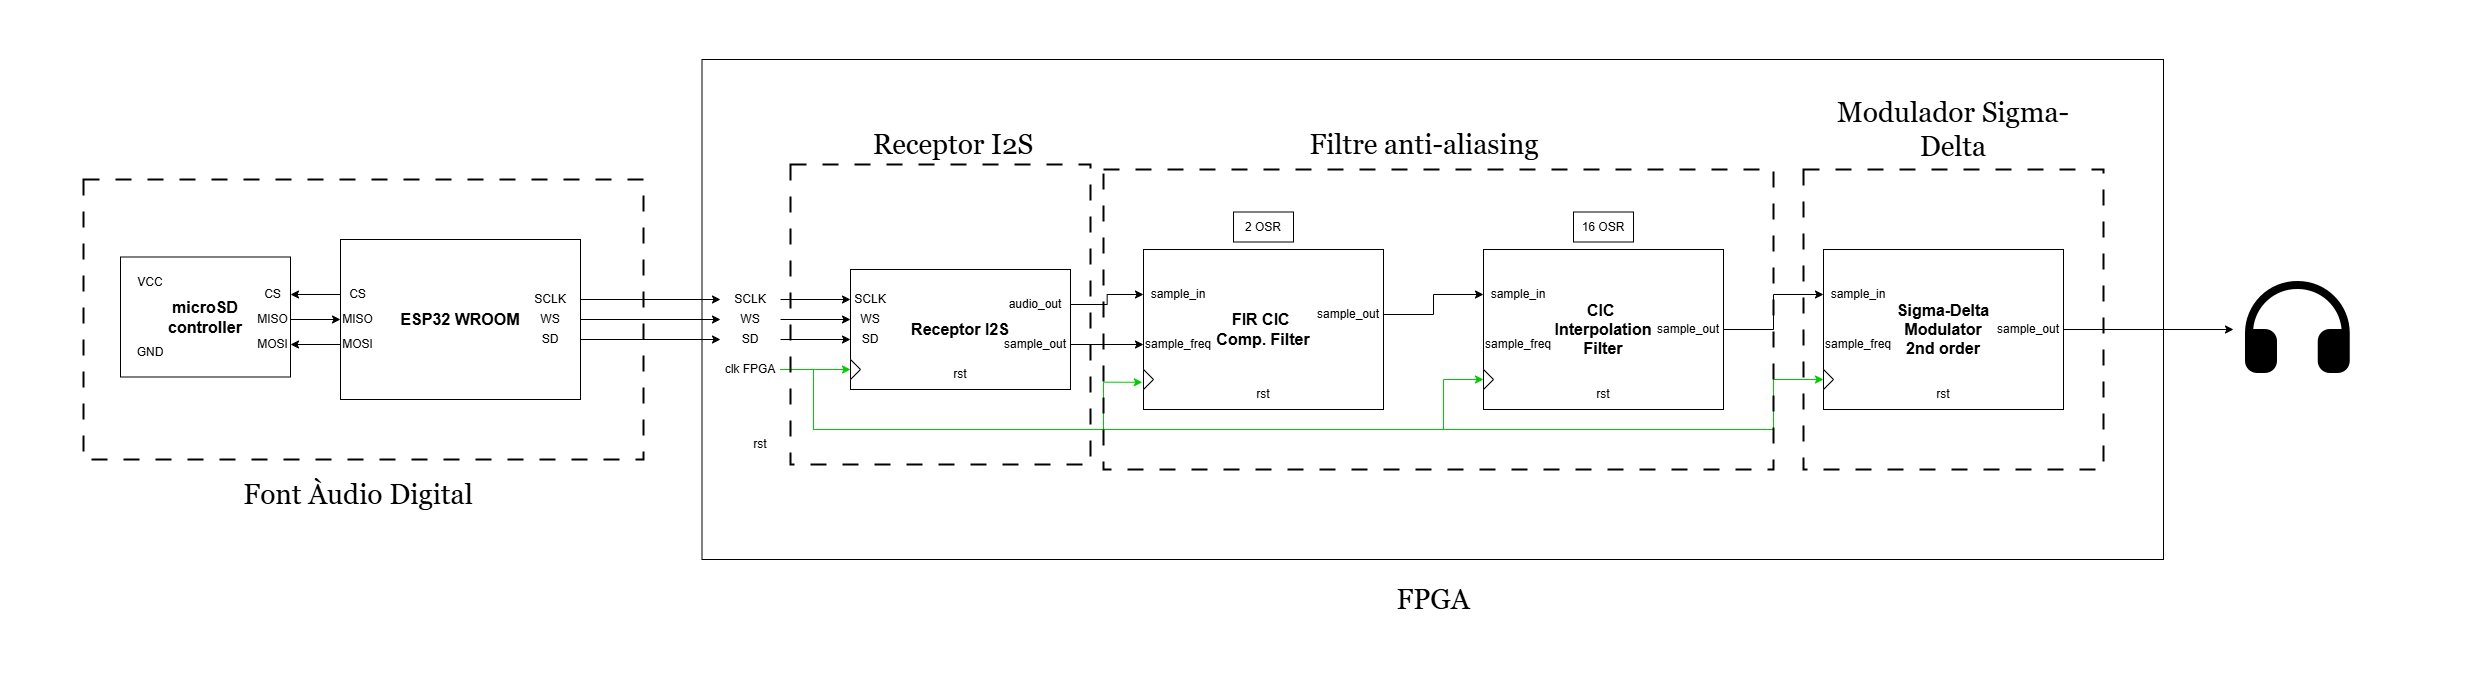
\includegraphics[angle=90,origin=c, width=0.4\linewidth]{Images/EstatActualTFG.drawio.png}
    \caption{Diagrama de blocs del sistema implementat en aquest treball.}
    \label{figTFGDiagr}
\end{figure}

\section{Font d'àudio en protocol I2S}
\par Per poder validar el funcionament de l'amplificador digital cal tenir una font d'àudio que transmeti en protocol I2S. Degut a que aquest protocol s'utilitza en comunicacions entre ICs, s'ha hagut d'implementar una entrada d'àudio que mantingui el protocol amb una targeta externa a la placa de desenvolupament. S'ha utilitzat una $\mu$SD per emmagatzemar els archius d'àudio .wav.

\section{Receptor d'àudio en protocol I2S}
\par S'ha implementat una entitat receptora en protocol I2S per captar les trames que s'envien pel bus. Aquest bloc és la primera etapa en el sistema implementat a la FPGA, i transmet el senyal internament a l'etapa de filtre anti-aliasing. El bloc està configurat per captar trames en mode d'operació estàndard Philips (veure apartat Protocol Inter-Integrated Sound).

\section{Etapa de filtrat anti-aliasing}
\par Com s'estudiarà més endavant, el filtre anti-aliasing s'implementa amb l'objectiu de mitigar l'acoblament d'imatges de freqüències més altes que la de mostreig, a l'espectre d'interés del senyal. En aquest treball es realitza l'etapa de filtrat en dos sub-blocs per efectuar l'etapa de sobre-mostreig de forma que no afecti a la qualitat del senyal.

\section{Modulador $\Sigma\Delta$}
\par L'última etapa de l'amplificador digital d'àudio de classe D desenvolupat en aquest treball és la del modelat de soroll. En el present treball la modelació del soroll de quantificació es realitza amb un bloc $\Sigma\Delta$ de segon ordre. 